% Author: Natasha T. Petrus
% Document type: Resume

\documentclass[letterpage]{article}

%%%%%%%%%%%%%%%%%%%%%%%%%%%%%%%%%%%%%
% DEFINE DEFAULT FONT STYLE
%%%%%%%%%%%%%%%%%%%%%%%%%%%%%%%%%%%%%
\usepackage{fontawesome}
\usepackage[defaultsans]{cantarell}
\usepackage[default,scale=0.95]{carlito}
\usepackage[T1]{fontenc}
\fontsize{10px}{0.45px}\selectfont
\usepackage{lmodern}

%%%%%%%%%%%%%%%%%%%%%%%%%%%%%%%%%%%%%
% DEFINE PAGE LAYOUT & SPACING
%%%%%%%%%%%%%%%%%%%%%%%%%%%%%%%%%%%%%
% For NO HYPHEN
\tolerance=1
\emergencystretch=\maxdimen
\hyphenpenalty=10000
\hbadness=10000
% NO HYPHEN END
\usepackage[top=0.55in, bottom=0.55in, left=0.55in,
right=0.85in]{geometry}
\usepackage{setspace} % for line spacing
\usepackage{vwcol} % unused - for columns with different widths
\usepackage{multicol} % unused - for columns with equal widths
% currently using minipage to create columns
\usepackage{enumitem} % for 'itemize' configuration
% http://ctan.org/pkg/enumitem

%%%%%%%%%%%%%%%%%%%%%%%%%%%%%%%%%%%%%
% COLOR PACKAGE & PREDEFINED COLORS
%%%%%%%%%%%%%%%%%%%%%%%%%%%%%%%%%%%%%
\usepackage[dvipsnames]{xcolor}
\definecolor{white-smoke}{HTML}{F2F7F8}
\definecolor{arsenic}{HTML}{40424A}
\definecolor{light-sky-blue}{HTML}{87CBFF}
\pagecolor{white-smoke}
\AtBeginDocument{\color{arsenic}}

%%%%%%%%%%%%%%%%%%%%%%%%%%%%%%%%%%%%%
% OTHER PACKAGES
%%%%%%%%%%%%%%%%%%%%%%%%%%%%%%%%%%%%%
\usepackage{verbatim} % for multi-line comments
\usepackage{graphicx} % for rotating text boxes
\usepackage{tikz} % for drawing shapes & highlights
\usepackage{soul} % for text highlights/underlines
\setul{-0.5ex}{1ex} % set underline dimension
\setuloverlap{3pt} % how much line is sticking out
\setulcolor{light-sky-blue}
\usepackage{amssymb,amsmath}
\usepackage{mathabx} % for math symbols
\usepackage{ifxetex,ifluatex}
\usepackage{fixltx2e} % provides \textsubscript
\ifnum 0\ifxetex 1\fi\ifluatex 1\fi=0 % if pdftex
  \usepackage[T1]{fontenc}
  % Setup & declare Unicode characters
  \usepackage[utf8]{inputenc}
  \DeclareUnicodeCharacter{0160}{\^--}
\else % if luatex or xelatex
  \ifxetex
    \usepackage{mathspec}
  \else
    \usepackage{fontspec}
  \fi
  \defaultfontfeatures{Ligatures=TeX,Scale=MatchLowercase}
\fi
% use upquote if available, for straight quotes in verbatim
% environments
\IfFileExists{upquote.sty}{\usepackage{upquote}}{}
% use microtype if available
\IfFileExists{microtype.sty}{%
\usepackage{microtype}
\UseMicrotypeSet[protrusion]{basicmath}
% ^ disable protrusion for tt fonts
}{}
\usepackage[unicode=true]{hyperref}
\hypersetup{
            pdfborder={0 0 0},
            breaklinks=true}
\urlstyle{same}  % don't use monospace font for urls
\usepackage{graphicx,grffile} % for inserting pictures
\makeatletter
\def\maxwidth{\ifdim\Gin@nat@width>\linewidth\linewidth\else
\Gin@nat@width\fi}
\def\maxheight{\ifdim\Gin@nat@height>\textheight\textheight\else
\Gin@nat@height\fi}
\makeatother
% Scale images if necessary, so that they will not overflow 
% the page margins by default, and it is still possible to
% overwrite the defaults using explicit options in
% \includegraphics[width,height, ...]{}
\setkeys{Gin}{width=\maxwidth,height=\maxheight,keepaspectratio}
\IfFileExists{parskip.sty}{%
\usepackage{parskip}
}{% else
\setlength{\parindent}{0pt}
\setlength{\parskip}{6pt plus 2pt minus 1pt}
}
\setlength{\emergencystretch}{3em}  % prevent overfull lines
\providecommand{\tightlist}{%
  \setlength{\itemsep}{0pt}\setlength{\parskip}{0pt}}
\setcounter{secnumdepth}{0}
% Redefines (sub)paragraphs to behave more like sections
\ifx\paragraph\undefined\else
\let\oldparagraph\paragraph
\renewcommand{\paragraph}[1]{\oldparagraph{#1}\mbox{}}
\fi
\ifx\subparagraph\undefined\else
\let\oldsubparagraph\subparagraph
\renewcommand{\subparagraph}[1]{\oldsubparagraph{#1}\mbox{}}
\fi

\begin{document}
\thispagestyle{empty} % to remove page number
%%%%%%%%%%%%%%%%%%%%%%%%%%%%%%%%%%%%%
% HEADER: NAME & INFOMARTION
%%%%%%%%%%%%%%%%%%%%%%%%%%%%%%%%%%%%%
\begin{minipage}[]{0.4\linewidth}
\raggedright
\textbf{\fontsize{37px}{1px}\selectfont\textsf{NATASHA}}\\
\vspace{7px}
{\fontsize{37px}{1px}\selectfont\textsf{PETRUS}}
\end{minipage}
\begin{minipage}{0.01\linewidth}
% INTENTIONALLY LEFT BLANK
\end{minipage}
\:\:\:\:\: % space between minipages
\begin{minipage}{0.33\linewidth}
\raggedleft
\vspace{5px} % for formatting purpose
natashapetr.us\enspace\faGlobe\\
hire@npetr.us\enspace\faPaperPlane\\
linkedin.npetr.us\enspace\faLinkedin\\
github.npetr.us\enspace\faGithubAlt
\end{minipage}
\:\:\:\:\: % space between minipages
\begin{minipage}[]{0.2\linewidth}
  \raggedright
  \begin{tikzpicture}
    \fill[light-sky-blue] (0,2.2) circle (1.2);
    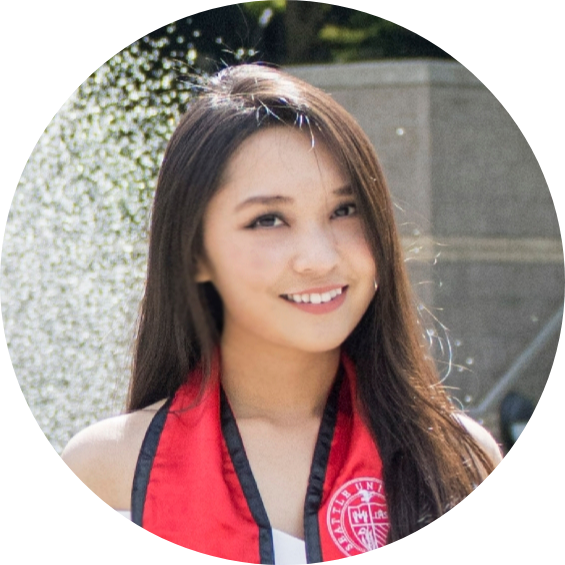
\includegraphics[width=1\linewidth]{assets/images/profile.png}
  \end{tikzpicture}
\end{minipage}
\vspace*{10px}\\ % space between header and content
%------------------------------------
% First Column
%------------------------------------
\begin{minipage}[t]{0.424\linewidth}
\vspace{0pt}
%%%%%%%%%%%%%%%%%%%%%%%%%%%%%%%%%%%%%
% EDUCATION HISTORY
%%%%%%%%%%%%%%%%%%%%%%%%%%%%%%%%%%%%%

\textbf{\fontsize{14px}{1px}\selectfont
  \ul{E D U C A T I O N}
}\\
\vspace{5px}\\
\textcolor{gray}{September 2015 - June 2017}\\
\textbf{\textsf{Seattle University - Seattle, WA}}\\
\textbf{Bachelor of Science in Electrical Engineering}\\
\textbf{Summa Cum Laude}\\
\textbf{GPA: 3.99 / 4.00}
\begin{itemize}[leftmargin=*,labelindent=5mm,labelsep=7mm]
\renewcommand\labelitemi{\rule[1mm]{0.33mm}{0.33mm}}
\renewcommand\labelitemii{$\blacksquare$}
\item
  Messina Merit Scholarship
  \begin{comment}
  {\begin{list}{}{} % to create indentation (w/o bulletpoints)
    \item
      For transfer student with
    \item
      minimum GPA of 3.75
  \end{list}}
  \end{comment}
\item
  IEEE-HKN Mu Iota Chapter
  {\begin{list}{}{}
    \item
    	Web Correspondent
  \end{list}}
\item
  Alpha Sigma Nu Jesuit Honor Society
  {\begin{list}{}{}
    \item
      Top 4\% of Senior Class
  \end{list}}
\item
  Tau Beta Pi Engineering Honor Society
\item
  Tau Sigma National Honor Society
\item
  President's and Dean's Lists
  {\begin{list}{}{}
    \item
    	September 2015 - June 2017
  \end{list}}
\end{itemize}
\vspace{7px}

%% College
\textcolor{gray}{September 2013 - June 2015}\\
\textbf{\textsf{North Seattle College - Seattle, WA}}\\
\textbf{Associate of Science Degree }

%\begin{itemize}[leftmargin=*,labelindent=5mm,labelsep=7mm]
%\renewcommand\labelitemi{\rule[1mm]{0.33mm}{0.33mm}}
%\renewcommand\labelitemii{$\blacksquare$} 
%\item
%  Phi Theta Kappa Honor Society
%  {\begin{list}{}{}
%    \item
%    	March 2014 - Present
%  \end{list}}
%\item
%  Vice President/Dean's List\\
%  September - December 2013
%\item
%  President's List\\
%  January 2014 - June 2015
%\end{itemize}
\vspace{19px}

%%%%%%%%%%%%%%%%%%%%%%%%%%%%%%%%%%%%%
% TECHNICAL SKILLS
%%%%%%%%%%%%%%%%%%%%%%%%%%%%%%%%%%%%%
\textbf{\fontsize{14px}{1px}\selectfont
  \ul{S K I L L S}
}\\
\vspace{0px}\\
\begin{minipage}[t]{0.01\linewidth}
% INTENTIONALLY LEFT BLANK
\end{minipage}
\: % space between left margin and text

\begin{minipage}[]{0.85\linewidth}
\raggedright
%\linespread{0.895}\selectfont
\textcolor{gray}{Software and Platforms:}
\begin{itemize}[label={},leftmargin=*,labelindent=5mm]
\item
Visual Studio,
GitHub/GitLab,
Jenkins,
Redis,
RabbitMQ,
Expo,
MS Office,
NI Multisim,
NI Ultiboard,
NI LabView,
Eclipse,
AutoCAD, 
Solidworks
\end{itemize}
\vspace{7px}
\textcolor{gray}{Languages, Libraries, and Frameworks:}\\
\begin{itemize}[label={},leftmargin=*,labelindent=5mm]
\item
C\#,
Selenium,
NUnit,
React Native,
ReactJS,
JavaScript
Typescript,
jQuery,
Knockout,
MATLAB,
LaTeX,
HTML,
CSS,
C,
C++,
VHDL,
Python,
MIPS Assembly Language,
Java,
PHP,
AngularJS,
SQL (MySql)
\end{itemize}
\vspace{7px}
\textcolor{gray}{Additional Skills:}
\begin{itemize}[leftmargin=*,labelindent=5mm,labelsep=7mm]
\renewcommand\labelitemi{\rule[1mm]{0.33mm}{0.33mm}}
\renewcommand\labelitemii{$\blacksquare$} 
\item
  Mobile app design and development
\item
  Full-stack web development
\item
  REST API development
\item
  PCB design, testing, and soldering
\item
  Custom IC layout design and testing
  \begin{comment}(starting from
  transistor level)\end{comment}
\item
  FPGA programming and testing
\item
  @RISK for financial analysis
\item
  Technical writing skills
\item
  Strong organizational, analytical, interpersonal,
  and presentation skills
\item
  Fast learner and a problem solver
\item
  Experienced in graphic design
\end{itemize}
\end{minipage}

%% !!!!!!! OLD VERSION 2 (NO COMPETENCY BARS)
%% NO ADDITIONAL SKILLS
\begin{comment}
\begin{minipage}[]{0.6\linewidth}
\linespread{0.895}\selectfont

\begin{multicols}{2}
\raggedright
%{\large \textcolor{gray}{SOFTWARE:}\:\:}\\
{\LARGE \rotatebox{90}{\textcolor{lightgray}{S O F T W A R E}}}\\
\columnbreak
Adobe Audition\\
Adobe Illustrator\\
Adobe Photoshop\\
AutoCAD\\
iATS Payments\\
Logisim\\
LTSpice\\
MS Access\\
MS Excel\\
MS PowerPoint\\
MS Publisher\\
MS Word\\
NI LabView\\
NI Ultiboard\\
Salesforce
% --------------------------------------------
\\~\\ % --------------LINE BREAK--------------
% --------------------------------------------
\end{multicols}
\end{minipage}

\begin{minipage}[]{0.6\linewidth}
\linespread{0.895}\selectfont

\begin{multicols}{2}
\raggedright
%{\large \textcolor{gray}{LANGUAGES:}}\\
{\LARGE \rotatebox{90}{\textcolor{lightgray}{L A N G U A G E S}}}\\
\columnbreak
C/C++\\
CSS\\
HTML\\
Java\\
Javascript\\
LaTeX\\
MATLAB\\
MIPS Assembly\\
PHP\\
Python\\
VHDL
\end{multicols}
\end{minipage}%
\end{comment}

%% !!!!!!! OLD VERSION (COMPETENCY BARS)
\begin{comment}
%------------------------------------
% First Sub-Column
%------------------------------------
\begin{minipage}[t]{0.33\linewidth}
\linespread{0.895}\selectfont % line spacing - SAME AS BELOW
\raggedleft
Adobe Audition\\
Adobe Illustrator\\
Adobe Photoshop\\
AutoCAD\\
iATS Payments\\
Logisim\\
LTSpice\\
MS Access\\
MS Excel\\
MS PowerPoint\\
MS Publisher\\
MS Word\\
NI LabView\\
NI Ultiboard\\
Salesforce
% --------------------------------------------
\\~\\ % --------------LINE BREAK--------------
% --------------------------------------------
C/C++\\
CSS\\
HTML\\
Java\\
Javascript\\
LaTeX\\
MATLAB\\
MIPS Assembly\\
PHP\\
Python\\
VHDL
\end{minipage}%
%------------------------------------
% Second Sub-Column
%------------------------------------
\:\:\: % space between text and bar
\begin{minipage}[t]{0.6\linewidth}
\linespread{0.895}\selectfont % line spacing - SAME AS LEFT COL.
% Adobe Audition:
\begin{tikzpicture}
\fill[black!10!white] (0,0.57) rectangle (2.9,0.35);
\fill[black!77!white] (0,0.57) rectangle (1.8,0.35);
\end{tikzpicture}\\
% Adobe Illustrator:
\begin{tikzpicture}
\fill[black!10!white] (0,0.57) rectangle (2.9,0.35);
\fill[black!77!white] (0,0.57) rectangle (1.1,0.35);
\end{tikzpicture}\\
% Adobe Photoshop:
\begin{tikzpicture}
\fill[black!10!white] (0,0.57) rectangle (2.9,0.35);
\fill[black!77!white] (0,0.57) rectangle (2.2,0.35);
\end{tikzpicture}\\
% AutoCAD:
\begin{tikzpicture}
\fill[black!10!white] (0,0.57) rectangle (2.9,0.35);
\fill[black!77!white] (0,0.57) rectangle (2.5,0.35);
\end{tikzpicture}\\
% iATS Payments:
\begin{tikzpicture}
\fill[black!10!white] (0,0.57) rectangle (2.9,0.35);
\fill[black!77!white] (0,0.57) rectangle (2.7,0.35);
\end{tikzpicture}\\
% Logisim:
\begin{tikzpicture}
\fill[black!10!white] (0,0.57) rectangle (2.9,0.35);
\fill[black!77!white] (0,0.57) rectangle (2.9,0.35);
\end{tikzpicture}\\
% LTSpice:
\begin{tikzpicture}
\fill[black!10!white] (0,0.57) rectangle (2.9,0.35);
\fill[black!77!white] (0,0.57) rectangle (2.9,0.35);
\end{tikzpicture}\\
% MS Access:
\begin{tikzpicture}
\fill[black!10!white] (0,0.57) rectangle (2.9,0.35);
\fill[black!77!white] (0,0.57) rectangle (1.7,0.35);
\end{tikzpicture}\\
% MS Excel:
\begin{tikzpicture}
\fill[black!10!white] (0,0.57) rectangle (2.9,0.35);
\fill[black!77!white] (0,0.57) rectangle (2.6,0.35);
\end{tikzpicture}\\
% MS PowerPoint:
\begin{tikzpicture}
\fill[black!10!white] (0,0.57) rectangle (2.9,0.35);
\fill[black!77!white] (0,0.57) rectangle (2.9,0.35);
\end{tikzpicture}\\
% MS Publisher:
\begin{tikzpicture}
\fill[black!10!white] (0,0.57) rectangle (2.9,0.35);
\fill[black!77!white] (0,0.57) rectangle (2.4,0.35);
\end{tikzpicture}\\
% MS Word:
\begin{tikzpicture}
\fill[black!10!white] (0,0.57) rectangle (2.9,0.35);
\fill[black!77!white] (0,0.57) rectangle (2.9,0.35);
\end{tikzpicture}\\
% NI LabView:
\begin{tikzpicture}
\fill[black!10!white] (0,0.57) rectangle (2.9,0.35);
\fill[black!77!white] (0,0.57) rectangle (2.0,0.35);
\end{tikzpicture}\\
% NI Ultiboard:
\begin{tikzpicture}
\fill[black!10!white] (0,0.57) rectangle (2.9,0.35);
\fill[black!77!white] (0,0.57) rectangle (2.0,0.35);
\end{tikzpicture}\\
% Salesforce:
\begin{tikzpicture}
\fill[black!10!white] (0,0.57) rectangle (2.9,0.35);
\fill[black!77!white] (0,0.57) rectangle (2.8,0.35);
\end{tikzpicture}
% --------------------------------------------
\\~\\ % --------------LINE BREAK--------------
% --------------------------------------------
% C/C++:
\begin{tikzpicture}
\fill[black!10!white] (0,0.57) rectangle (2.9,0.35);
\fill[black!77!white] (0,0.57) rectangle (2.4,0.35);
\end{tikzpicture}\\
% CSS:
\begin{tikzpicture}
\fill[black!10!white] (0,0.57) rectangle (2.9,0.35);
\fill[black!77!white] (0,0.57) rectangle (2.6,0.35);
\end{tikzpicture}\\
% HTML:
\begin{tikzpicture}
\fill[black!10!white] (0,0.57) rectangle (2.9,0.35);
\fill[black!77!white] (0,0.57) rectangle (2.9,0.35);
\end{tikzpicture}\\
% Java:
\begin{tikzpicture}
\fill[black!10!white] (0,0.57) rectangle (2.9,0.35);
\fill[black!77!white] (0,0.57) rectangle (2.0,0.35);
\end{tikzpicture}\\
% Javascript:
\begin{tikzpicture}
\fill[black!10!white] (0,0.57) rectangle (2.9,0.35);
\fill[black!77!white] (0,0.57) rectangle (1.3,0.35);
\end{tikzpicture}\\
% LaTeX:
\begin{tikzpicture}
\fill[black!10!white] (0,0.57) rectangle (2.9,0.35);
\fill[black!77!white] (0,0.57) rectangle (2.0,0.35);
\end{tikzpicture}\\
% MATLAB:
\begin{tikzpicture}
\fill[black!10!white] (0,0.57) rectangle (2.9,0.35);
\fill[black!77!white] (0,0.57) rectangle (2.8,0.35);
\end{tikzpicture}\\
% MIPS Assembly:
\begin{tikzpicture}
\fill[black!10!white] (0,0.57) rectangle (2.9,0.35);
\fill[black!77!white] (0,0.57) rectangle (2.3,0.35);
\end{tikzpicture}\\
% PHP:
\begin{tikzpicture}
\fill[black!10!white] (0,0.57) rectangle (2.9,0.35);
\fill[black!77!white] (0,0.57) rectangle (1.8,0.35);
\end{tikzpicture}\\
% Python:
\begin{tikzpicture}
\fill[black!10!white] (0,0.57) rectangle (2.9,0.35);
\fill[black!77!white] (0,0.57) rectangle (2.6,0.35);
\end{tikzpicture}\\
% VHDL:
\begin{tikzpicture}
\fill[black!10!white] (0,0.57) rectangle (2.9,0.35);
\fill[black!77!white] (0,0.57) rectangle (2.3,0.35);
\end{tikzpicture}
\end{minipage}
\end{comment}

\end{minipage}%
%------------------------------------
% Second Column
%------------------------------------
\begin{minipage}[t]{0.63\linewidth}
\vspace{0pt}
%%%%%%%%%%%%%%%%%%%%%%%%%%%%%%%%%%%%%
% RELEVANT EXPERIENCE
%%%%%%%%%%%%%%%%%%%%%%%%%%%%%%%%%%%%%
\textbf{\fontsize{14px}{1px}\selectfont
  \ul{R E L E V A N T \:\: E X P E R I E N C E}
}\\

%% Geniuslink: Software Engineer
\vspace{7px}
\textcolor{gray}{October 2017 - Present}\\
\textbf{\textsf{Software Engineer at Geniuslink}}
\begin{itemize}[leftmargin=*,labelindent=1mm,labelsep=0mm]
\renewcommand\labelitemi{\rule[1mm]{0.33mm}{0.33mm}}
\renewcommand\labelitemii{$\blacksquare$}
\item
  \begin{quote}
  \raggedright
  Has increased the number of integration tests against the company's whole web
  application and service by more than 3000\% thus far
  \end{quote}
\item
  \begin{quote}
  \raggedright
  Constantly automating tests using Jenkins/Mono,
  Selenium (C\#), NUnit, and ServiceStack
  \end{quote}
\item
  \begin{quote}
  \raggedright
  Allowed all integration tests to be run against any
  environment easily through Jenkins and greatly
  assisted in making Canary testing possible
  \end{quote}
\item
  \begin{quote}
  \raggedright
  Mocked third-party APIs for testing against the company's service
  \end{quote}
\item
  \begin{quote}
  \raggedright
  Designed and developed Geniuslink's REST API v3
  \end{quote}
\item
  \begin{quote}
  \raggedright
  Designed and programmed the preliminary version of the company's mobile
  application using React Native
  \end{quote}
\item
  \begin{quote}
  \raggedright
  Frontend/backend work using C\#, Typescript/JS,
  jQuery, and Knockout
  \end{quote}
\end{itemize}

%% HCI Technologies/Microsoft: Game Tester
\vspace{7px}
\textcolor{gray}{September - October 2017}\\
\textbf{\textsf{Game Tester at HCL Technologies/Microsoft}}\\
\raggedright
Worked within HCL Technologies' CERT lab to certify pre-released
games and the DLCs were up to specified software and platform standards.

%% Senior Design / Interdisciplinary Project: T-Mobile
\vspace{7px}
\textcolor{gray}{
  {\small[PATENT PENDING]\enspace}
  September 2016 - June 2017}\\
\textbf{\textsf{Interdisciplinary Project:
		T-Mobile Compact Robotic System}}\\
\raggedright
Refined handset validation testing for T-Mobile via robotic
implementation;\\reduced manufacturing cost by at least 50\%,
reduced physical size by at least 60\%, and improved
power efficiency.\\
\begin{itemize}[leftmargin=*,labelindent=1mm,labelsep=0mm]
\renewcommand\labelitemi{\rule[1mm]{0.33mm}{0.33mm}}
\renewcommand\labelitemii{$\blacksquare$}
\item
  \begin{quote}
  \raggedright
  Designed and manufactured two working prototypes within
  a year using SolidWorks (3D modeling)
  \end{quote}
\begin{comment}
\item
  \begin{quote}
  \raggedright
  Processed data points gathered from single taps generated
  by the first prototype using MATLAB to generate margin of position
  error and to observe how much force is applied to device screen
  \end{quote}
\item
  \begin{quote}
  \raggedright
  Used MATLAB to generate the z-axis actuator positional feedback
  from thousands of data points
  \end{quote}
\item
  \begin{quote}
  \raggedright
  Used OpenCV to detect a signifier on the phone's GUI in order
  to ensure a certain test case is successfully passed
  \end{quote}
\end{comment}
\item
  \begin{quote}
  \raggedright
  Programmed in C++,
  used OpenCV and LabView for image processing
  \end{quote}
\end{itemize}

%% VLSI Project: 4-bit ALU
\vspace{7px}
\textcolor{gray}{March - June 2017}\\
\textbf{\textsf{VLSI Project: ALU Integrated Circuit Design}}\\
\raggedright
Designed the 3D layout of an ALU chip from transistor level
using Electric VLSI.

%% Independent Study Project
\vspace{7px}
\textcolor{gray}{January - March 2017}\\
\textbf{\textsf{Independent Study: 13.56MHz RFID on Ettus N210 SDR}}\\
\raggedright
Implemented the ISO 18000 13.56 MHz RFID standard on software defined
radios with LFRX and LFTX daughterboards.
\begin{comment}
\begin{itemize}[leftmargin=*,labelindent=1mm,labelsep=0mm]
\renewcommand\labelitemi{\rule[1mm]{0.33mm}{0.33mm}}
\renewcommand\labelitemii{$\blacksquare$}
\item
  \begin{quote}
  \raggedright
  Used MATLAB to generate modulated waves to test
  demodulation of self-built AM receiver and to generate
  waves to be transmitted by a tag reader to power RFID tags
  \end{quote}
\end{itemize}
\end{comment}

\begin{comment}
%% DSP
\vspace{7px}
\textcolor{gray}{September - December 2016}\\
\textbf{\textsf{SU Course Project: Digital Signal Processing}}\\
  \raggedright
  Used MATLAB and data sampling to manipulate sound waves,
  and to build and test different filters on MATLAB-generated
  waves.
\end{comment}

%% Aneka Elektrindo Panel
\vspace{7px}
\textcolor{gray}{July - August 2016}\\
\textbf{\textsf{Electrical Engineering Intern
at PT Aneka Elektrindo Panel}}\\
\raggedright
Designed and built circuit panels based on client's
specifications using AutoCAD.

%% Global Visionaries
\vspace{7px}
\textcolor{gray}{October 2015 - June 2016}\\
\textbf{\textsf{Internship: IT Manager at Global Visionaries}}\\
\begin{itemize}[leftmargin=*,labelindent=1mm,labelsep=0mm]
\renewcommand\labelitemi{\rule[1mm]{0.33mm}{0.33mm}}
\renewcommand\labelitemii{$\blacksquare$}
\item
  \begin{quote}
  \raggedright
  Set up an online auction and created a donation page to
  support the educational needs of underprivileged youth
  \end{quote}
\item
  \begin{quote}
  \raggedright
  Provided network security strategies and conducted staff
  training
  \end{quote}
\end{itemize}

%% ECE Junior Project: Automated Puppet Show
\begin{comment}
\vspace{7px}
\textcolor{gray}{September 2015 - June 2016}\\
\textbf{\textsf{ECE Junior Project: Automated Puppet Show}}\\
\raggedright
Built an automated puppet show using semiconductor devices and Raspberry Pi.
\end{comment}

%% MATLAB Tutor & Grader
\vspace{7px}
\textcolor{gray}{January - March 2016}\\
\textbf{\textsf{MATLAB Teaching Assistant at Seattle University}}
\begin{itemize}[leftmargin=*,labelindent=1mm,labelsep=0mm]
\renewcommand\labelitemi{\rule[1mm]{0.33mm}{0.33mm}}
\renewcommand\labelitemii{$\blacksquare$}
\item
  \begin{quote}
  \raggedright
  Provided in-class help and out-of-class tutoring sessions
  \end{quote}
\item
  \begin{quote}
  \raggedright
  Graded weekly projects and assignments
  \end{quote}
\end{itemize}

%% VHDL Project: Pong Game
\begin{comment}
\vspace{7px}
\textcolor{gray}{January - March 2016}\\
\textbf{\textsf{FPGA Project: Pong Game}}\\
\raggedright
Created game written in C and VHDL using Altera board,
Arduino, and VGA monitor.
\end{comment}

%% MATLAB Course Project
\begin{comment}
\vspace{7px}
\textcolor{gray}{September - December 2015}\\
\textbf{\textsf{SU MATLAB Course Small Project}}\\
\raggedright
Created Snakes and Ladders game on MATLAB for 2-4 players.
\end{comment}

\end{minipage}

\end{document}